\section{Technological Background}
% ADD high lever overviews of flink and kafka like execution engigne graph or kafka cluster%

\par In the last years, many systems for large-scale and distributed stream processing have been proposed, including Spark Streaming \cite{Spark},  Apache Storm \cite{Storm} and Apache Flink \cite{Flink}. These frameworks can ingest and process real-time data streams, published from different distributed message queuing platforms, such as Apache Kafka \cite{Kafka} or  Amazon Kinesis \cite{Kinesis}. 
\par In this thesis, we implemented the proposed system in Apache Flink. Flink provides the distributed stream processing components of the distributed event pattern predictors. It works alongside Apache Kafka, which is used for streaming the input event streams and as a messaging platform that enables the distributed online learning functionalities.


%\par In the datAcron project, the Flink streaming processing engine has been chosen as a primary platform for supporting the streaming operations, based on an internal comparative evaluation of several streaming platforms. Hence, we used it to implement our system. A predecessor distributed online learning framework has already been implemented in the FERARI project \cite{flouris2016ferari} based on Apache Storm.


% In Storm, a distributed application is expressed as a "topology", in which the individual processing steps called "Bolts" are connected
%in a data workflow. This means, that each Bolt can is sending and receiving data streams from other Bolts, for example, there are bolts generating
%the local models for each incoming data streams and there is a Bolt representing the "Coordinator" for executing the synchronization protocol between
%the local models. As the synchronization protocol includes the steps of sending the local models to the coordinator (for merging the models) and of sending
%the merged model back, it results in a cyclic workflow structure, which is supported in Storm. 

\subsection{Apache Flink}

\par Apache Flink is an open source project that provides a large-scale, distributed, and stateful stream processing platform \cite{carbone2015apache}. Flink is one of the most recent and pioneering Big Data processing frameworks.

\par  It provides processing models for both streaming and batch data, where the batch processing model is treated as a special case of the streaming one (i.e., finite stream). Flink's software stack includes the \textit{DataStream} and \textit{DataSet} APIs for processing infinite and finite data, respectively. These two core APIs are built on top of Flink's core dataflow engine and provide multiple operations on data streams or sets such as \textit{mapping}, \textit{filtering}, \textit{grouping}, etc.

\par The two main data abstractions of Flink are \textit{DataStream} and \textit{DataSet},  they represent read-only collections of data elements. The list of elements is bounded (i.e., finite) in \textit{DataSet}, while it is unbounded (i.e., infinite) in the case of \textit{DataStream}. Flink's core is a distributed streaming dataflow engine. 


\par Flink programs are represented by a data-flow graphs (i.e., directed acyclic graph - DAG) that get executed by Flink's dataflow engine \cite{carbone2015apache}. The data flow graphs are composed of stateful operators and intermediate data stream partitions.  The execution of each operator is handled by multiple parallel instances whose number is determined by the \textit{parallelism} level. Each parallel operator instance is executed in an independent task slot on a machine within a cluster of computers \cite{Flink}.
\par  Figure~\ref{fig:flink} shows an example of data flow graph in for Flink's program.

\begin{figure}[H]
	\centering
	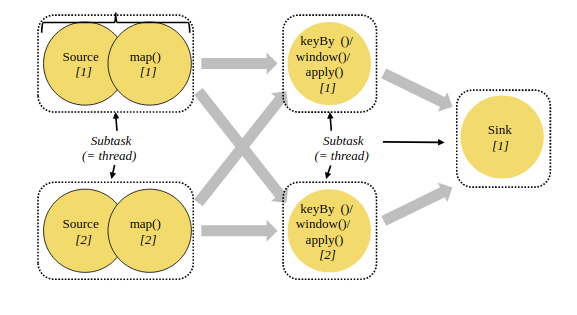
\includegraphics[width=\linewidth]{chapters/figures/flink_program.png}
	
	\caption{A parallel data flow graph in Flink \cite{Flink}.}
	\label{fig:flink}
\end{figure}
    

\subsection{Apache Kafka}

\par Apache Kafka is a scalable, fault-tolerant, and distributed streaming framework/messaging system \cite{Kafka}. It allows to publish and subscribe to arbitrary data streams, which are managed in different categories (i.e., \textit{topics}) and  partitioned in the Kafka cluster. 
\par The Kafka producer API provides the ability to publish a stream of messages to a topic. These messages can then be consumed by applications, using the Consumer \ac{api} that allows them to read the published data stream in the Kafka cluster. In addition, the streams of messages are distributed and load balanced between the multiple receivers within the same consumer group for the sake of scalability. In this work, we leverage the topic-based routing of the messages to control the communication that is required to perform the distributed online learning protocol. 
% (see Section ~\ref{sec:impl}).    
  





%The distributed online learning framework has already been implemented in the FERARI  distributed streaming architecture based on Storm. 
%In Storm, a distributed application is expressed as a so-called “topology”, in which the individual processing steps called “Bolts” are connected
%in a data workflow. This means, that each Bolt can is sending and receiving data streams from other Bolts, for example, there are bolts generating
%the local models for each incoming data streams and there is a Bolt representing the “Coordinatior” for executing the synchronisation protocol between
%the local models. As the synchronisation protocol includes the steps of sending the local models to the coordinator (for merging the models) and of sending
%the merged model back, it results in a cyclic workflow structure, which is supported in Storm. 
%
%Why Flink
%In the Datacron project, the Flink streaming engine has been chosen as primary platform for supporting the streaming operations, based on an internal comparative evaluation of several streaming platforms
%regarding functionality and performance. We will discuss in section.. how to implement the required communication structure for the distributed
%online learning framework in Flink.